\documentclass[tikz, border=0pt]{standalone}
\usepackage{tikz}
\usetikzlibrary{arrows,automata,positioning}

\begin{document}
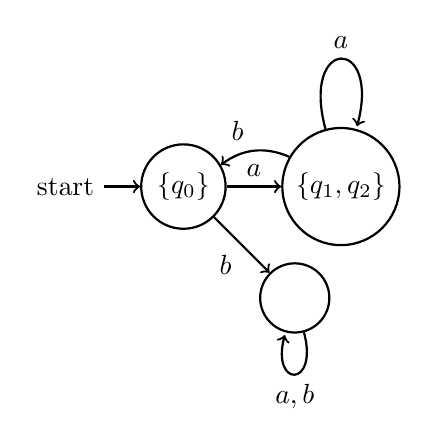
\begin{tikzpicture}[node distance=2cm, thick, auto]
% draw the states
\node[state, initial] (q_0) {\(\{q_0\}\)};
\node[state] (q_12) [right of=q_0] {\(\{q_1, q_2\}\)};
\node[state] (q_n) [below right of=q_0] {};
;
\path[->] 
(q_0) edge node {\(a\)} (q_12)
(q_0) edge node [swap] {\(b\)} (q_n)
(q_12) edge [loop above] node {\(a\)} (q_n)
(q_12) edge [bend right] node [swap] {\(b\)} (q_0)
(q_n) edge [loop below] node {\(a, b\)} (q_n)
;
\end{tikzpicture}
\end{document}